\chapter{Introduction}

\section{Context and Problem Definition}

Medication management is a high-stakes, complex process central to modern healthcare delivery. Its successful execution is critical for patient safety, yet it remains a major source of preventable adverse events. The landmark report "To Err is Human" by the Institute of Medicine brought global attention to the prevalence of medical errors, identifying them as a leading cause of morbidity and mortality \cite{kohn2000}. Subsequent research and initiatives by the World Health Organization have reinforced this reality, indicating that medication-related harm affects one in ten patients globally and that the associated costs are substantial \cite{who2017, who2022}.

A primary contributing factor to this problem is the fragmented nature of Health Information Technology (HIT) ecosystems within hospitals \cite{berwick2008}. Many healthcare institutions operate on a patchwork of legacy systems, often developed decades apart using disparate technologies \cite{kazemi2016}. This technological heterogeneity creates significant barriers to interoperability, resulting in information silos where critical patient data is not shared effectively between departments or professionals. This fragmentation directly undermines continuity of care and has been identified as a key threat to patient safety \cite{ash2004, keasberry2017}. The workflow, which should be a seamless continuum from a physician's prescription to pharmaceutical validation and finally to nursing administration, is often interrupted by manual processes, verbal communications, and data re-entry, each step introducing a new opportunity for error.

\begin{figure}[htbp]
    \centering
    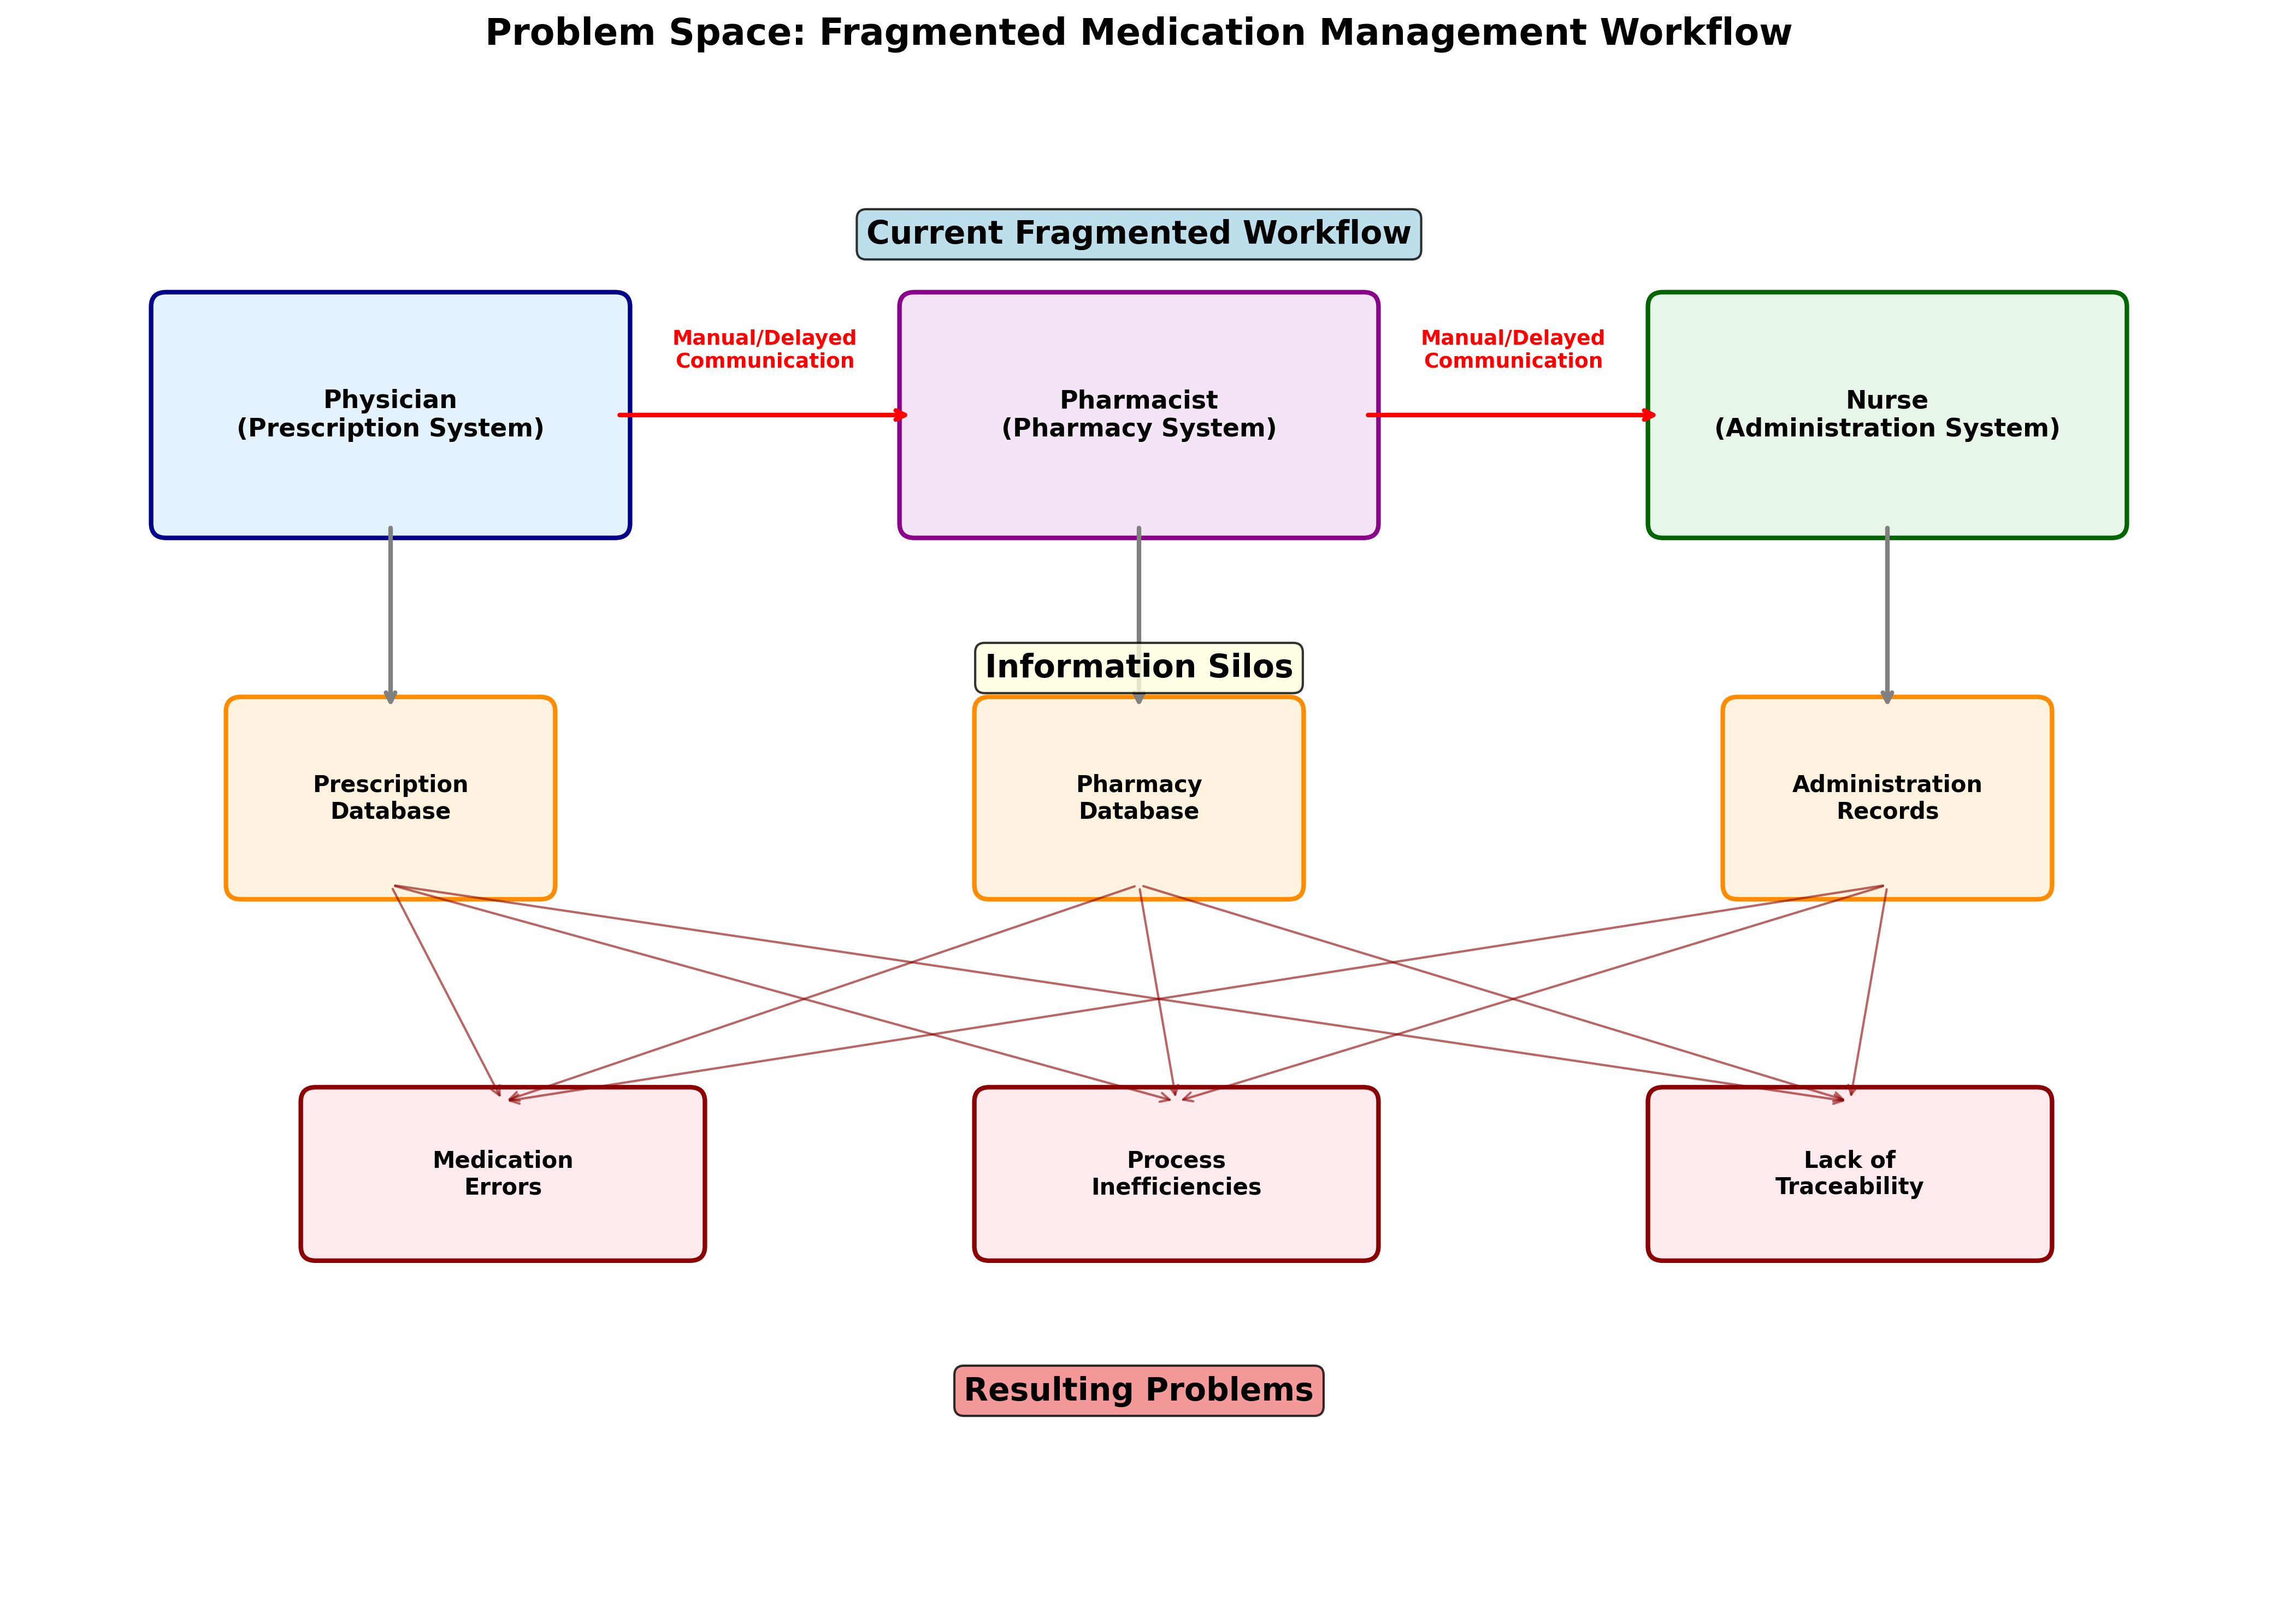
\includegraphics[width=0.9\textwidth]{images/generated/problem_space_diagram.png}
    \caption{Conceptual diagram of the problem space, illustrating the fragmented communication flow and resulting information silos that contribute to medication errors and operational inefficiencies.}
    \label{fig:problem_space}
\end{figure}

The Santa Casa da Misericórdia de Vila Verde (SCMVV) serves as a representative case study for these systemic challenges. Its core operations rely on the AIDA-PCE, a legacy system with significant limitations, including a non-intuitive interface, a lack of real-time clinical decision support (e.g., for drug interactions), and poor integration capabilities \cite{moss2015, bowles2020}. This environment compromises patient safety and hampers operational efficiency. This dissertation addresses these issues by detailing the design, development, and implementation of a modern, integrated medication management system aimed at creating a cohesive, safe, and efficient clinical workflow.

\section{Objectives and Dissertation Structure}

The primary goal of this research is to develop and evaluate an integrated medication management system that optimizes the prescription, validation, dispensing, and administration processes at the SCMVV, thereby enhancing patient safety and operational efficiency. To achieve this, a set of specific scientific and technological objectives was defined. Scientifically, the aim was to analyze the system's impact on medication error rates, evaluate its effect on clinical workflow efficiency, and assess its usability and acceptance among clinical staff. Technologically, the objectives were to design a scalable microservices architecture, develop a robust clinical decision support engine, create an intuitive user interface using modern web technologies, ensure seamless integration with legacy systems, and establish a comprehensive audit trail for all medication-related activities \cite{belle2013, misra2023, mandl2020, european2016}.

This dissertation is organized to logically present the research journey. Following this introduction, Chapter 2 provides a comprehensive review of the State of the Art. Chapter 3 outlines the Work Plan, detailing the project's timeline and phases. Chapter 4 describes the in-depth research Methodology, including the architectural choices and evaluation strategies. Chapter 5 presents the Results from the system's implementation and pilot study. Chapter 6 offers a Discussion of these results, contextualizing them within the broader literature. Finally, Chapter 7 provides the Conclusion, summarizing the contributions and proposing directions for future work. 